%\documentclass[hyperref={pdfpagelabels=false}]{beamer}
\documentclass{beamer}

\usepackage{beamerthemeSingapore}
%\usepackage{beamerthemebars}
%\usepackage{algorithmic}
%\usepackage{algorithm}
%\usepackage{graphicx}
%\usepackage{subfigure}
\usepackage{url}
%\usecolortheme{orchid}

\title{Ensemble Method for Spam Classification}
\author{Hannu Hartikainen and Eric Malmi}
%\institute{Helsinki Institute of Physics / Adaptive Informatics Research Centre, \\ Aalto University (Helsinki University of Technology)}

\date{\today}

\setbeamertemplate{footline}[page number]
\begin{document}

\setlength{\unitlength}{\textwidth}

\frame{\titlepage}
%\frame{\tableofcontents}
\frame{
\frametitle{Outline}
\begin{itemize}
  \item Introduction
  \item Self-Organizing Map
  \item Algorithms
  \begin{itemize}
    \item Neural Networks
    \item Support Vector Machines
    \item Gene Expression Programming
    \item Multi-class classification
  \end{itemize}
  \item Results
  \item Practical tips
\end{itemize}
}

\section{Methods}
\subsection{}

\frame
{
  \frametitle{Ensemble Method}

  \begin{itemize}
    \item Foo.
  \end{itemize}

%\begin{figure}
%	\centering
%	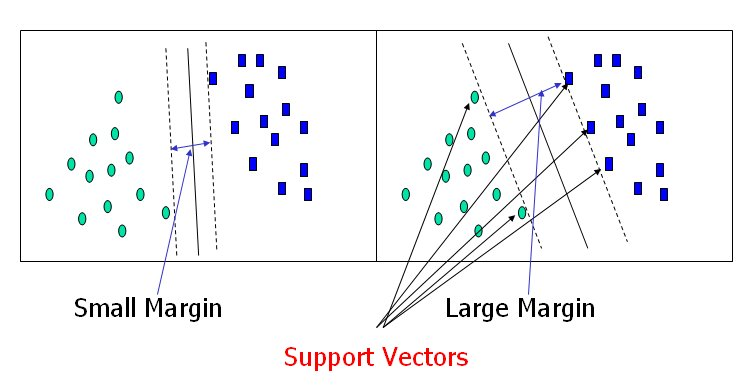
\includegraphics[width=\textwidth]{svm_margin.jpg}
	%\caption{Source:}
%\end{figure}
}

\frame
{
    \frametitle{Random Forest}

    \begin{figure}
        \centering
        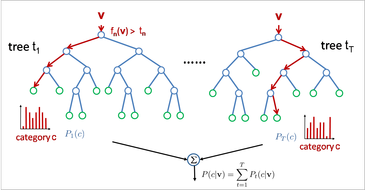
\includegraphics[width=0.7\textwidth]{random_forest_new2.png}
        %\caption{Source: http://www.iis.ee.ic.ac.uk/~tkkim/iccv09_tutorial}
    \end{figure}

    \begin{itemize}
        \item Ensemble classifier using $n$ random trees
        \begin{itemize}
            \item Pick random attributes for each tree node
            \item Calculate the best split using those attributes
        \end{itemize}
    \end{itemize}

}

\frame
{
  \frametitle{Support Vector Machine}

  \begin{itemize}
    \item Support Vector Machine (SVM) finds a hyperplane that separates two data samples with the largest possible margin 
  \end{itemize}

\begin{figure}
	\centering
	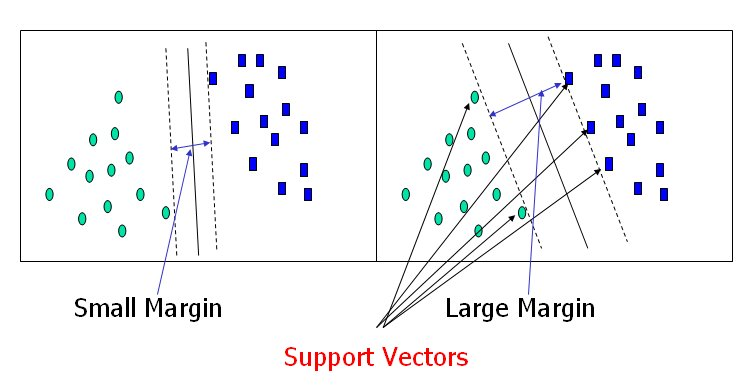
\includegraphics[width=\textwidth]{svm_margin.jpg}
	%\caption{Source:}
\end{figure}
}

\frame
{
  \frametitle{Support Vector Machines}

\begin{columns}
\begin{column}{7cm}
{\small
  \begin{itemize}
    \item Project data vectors nonlinearly into a higher dimensional space $\Rightarrow$ more probable to find a separating hyperplane (Cover's theorem)
    \item We only need to define the dot product, i.e. the kernel function $\Phi(x,y)$, in the high-dimensional space (the kernel trick)
    \item We use a popular radial basis function: $\Phi(x,y) = \exp(-\gamma||x-y||^2)$
  \end{itemize}
}
\end{column}
\begin{column}{4.5cm}
\begin{figure}
	\centering
		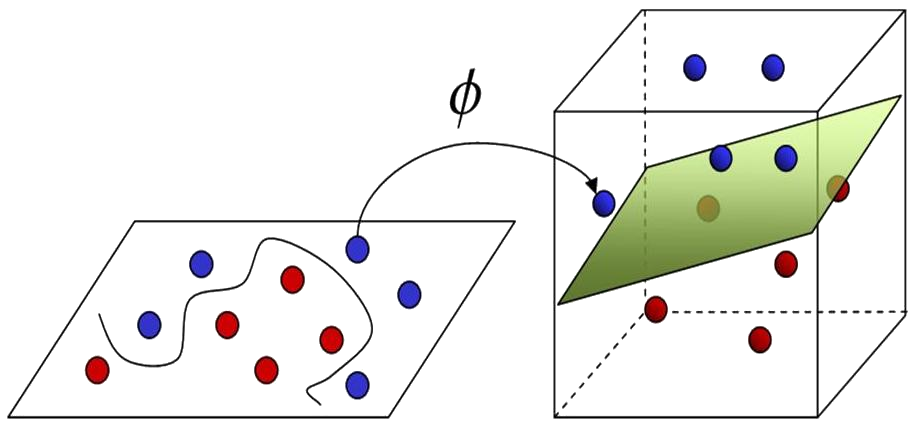
\includegraphics[width=\textwidth]{svm2.png}
	\label{fig:bridge}
\end{figure}
\end{column}
\end{columns}
}

\frame
{
  \frametitle{Bernoulli Mixture}

  \begin{itemize}
    \item Mixture of multivariate Bernoulli distributions
    %\item Natural for bivariate data, 
  \end{itemize}
  \begin{eqnarray*}
    p(\mathbf{x}|\boldsymbol\mu) &=& \prod_{i=1}^D \mu_i^{x_i}(1-\mu_i)^{(1-x_i)} \\
    p(\mathbf{x}|\boldsymbol\mu,\boldsymbol\pi) &=& \sum_{k=1}^K \pi_kp(\mathbf{x}|\boldsymbol\mu_k)
  \end{eqnarray*}
  \begin{itemize}
    \item Natural choise for bivariate data
    \item Outputs probabilities
    \item Can capture correlations between variables
  \end{itemize}

%\begin{figure}
%	\centering
%	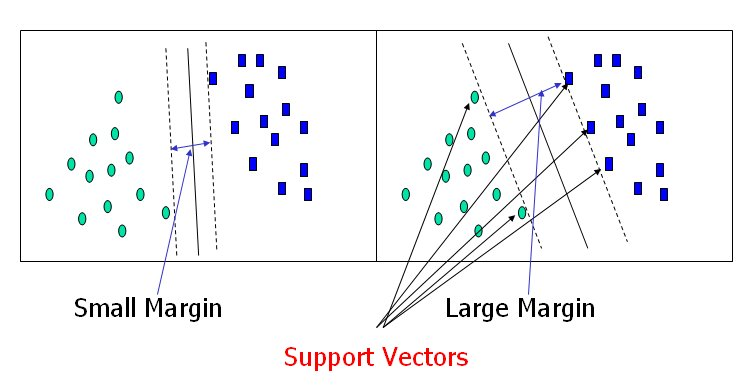
\includegraphics[width=\textwidth]{svm_margin.jpg}
	%\caption{Source:}
%\end{figure}
}

\section{Results}
\subsection{}
\frame
{
  \frametitle{Results}

Average efficiencies of different algorithms (left) and the performance of the NN ordered binarization (right). 

\begin{columns}
\begin{column}{4cm}

{\scriptsize
\begin{table}
\hspace{1.0cm}
%\caption{Average efficiencies of different algorithms}
%\begin{center}
\begin{tabular}{l|c}
Method & $<$Efficiency$>$ \\ \hline
GEP & 92.49 \\
%GEP one-against-all & 88.54 \\
SVM & 94.21 \\
%SVM one-against-one & 94.38 \\
NN & 94.54 \\
%NN 5 outputs & 94.42
\end{tabular}
%\end{center}
\end{table}
}
\end{column}
\begin{column}{7cm}

\hspace{2.2cm}
{\scriptsize
\begin{table}
%\caption{Performance of the NN ordered binarization.}
%\begin{center}
\begin{tabular}{c|cccc}
  Real\textbackslash Pred & DD & SD & CD & ND \\ \hline
  DD & {\bf 87.60} & 12.05 & 0.35 & 0.00 \\
  SD & 2.15 & {\bf 95.20} & 2.58 & 0.07 \\
  CD & 0.00 & 4.25 & {\bf 95.75} & 0.00 \\
  ND & 0.15 & 0.25 & 0.00 & {\bf 99.60} \\ \hline
  Purities &  {\bf 97.44} & {\bf 85.19} & {\bf 97.03} & {\bf 99.93}
\end{tabular}
%\end{center}
\end{table}
}
\end{column}

\end{columns}

The results have been obtained optimizing the total accuracy
(the probability that an event of random category is classified correctly)
}

\end{document}
